\documentclass[12pt,a4paper]{article}

\usepackage{fontspec}
\usepackage{polyglossia}
\setmainlanguage{russian}
\setotherlanguage{english}
\setmainfont{Liberation Serif}
\setsansfont{Liberation Sans}
\setmonofont{Liberation Mono}

\usepackage[a4paper,margin=2.5cm]{geometry}
\usepackage{graphicx}
\usepackage{float}
\usepackage{caption}
\usepackage{array}
\usepackage{longtable}
\usepackage{listings}
\usepackage{xcolor}
\usepackage{hyperref}
\usepackage{indentfirst}
\usepackage{setspace}

\onehalfspacing
\hypersetup{colorlinks=true, linkcolor=black, urlcolor=blue}

\lstdefinelanguage{JavaScript}{
  keywords={const,let,var,function,return,true,false,if,else},
  keywordstyle=\color{blue},
  comment=[l]{//},
  commentstyle=\color{gray},
  stringstyle=\color{red!60!black},
  morestring=[b]',
  morestring=[b]"
}

\lstset{
  basicstyle=\ttfamily\small,
  breaklines=true,
  frame=single,
  columns=fullflexible,
  keepspaces=true,
  showstringspaces=false,
  tabsize=2
}

\begin{document}

\begin{titlepage}
\begin{center}
САНКТ-ПЕТЕРБУРГСКИЙ НАЦИОНАЛЬНЫЙ\\
ИССЛЕДОВАТЕЛЬСКИЙ УНИВЕРСИТЕТ ИТМО\\
\vspace{0.5cm}
Дисциплина: Бэк-энд разработка

\vspace{4cm}
{\Large Отчет}\\
\vspace{0.3cm}
{\large Домашнее задание №3}\\
\vspace{0.3cm}
{\large Тестирование API средствами Postman}

\vfill
\begin{flushright}
Выполнил:\\
Катков Алексей Сергеевич\\
Группа K3339\\
Поток БР1.2\\
\vspace{0.5cm}
Проверил:\\
Добряков Давид Ильич
\end{flushright}

\vfill
Санкт-Петербург\\
2026 г.
\end{center}
\end{titlepage}

\section*{Задача}

Реализовать тестирование API средствами Postman и написать автотесты внутри Postman. В результате необходимо получить один комплексный сценарий по основному процессу в приложении.

В рамках работы тестировался API сервиса обмена рецептами и кулинарных блогов. Основной пользовательский сценарий был выбран следующим образом:

\begin{center}
\textit{регистрация пользователя $\rightarrow$ авторизация $\rightarrow$ создание рецепта $\rightarrow$ получение списка рецептов с фильтрацией $\rightarrow$ получение рецепта по идентификатору.}
\end{center}

\section*{Ход работы}

\subsection*{Описание тестируемого API}

Тестируемое приложение представляет собой серверную часть сервиса для публикации и просмотра кулинарных рецептов. В проекте используются Node.js, Express, TypeScript, PostgreSQL и TypeORM. Для авторизации пользователей применяется JWT-токен.

Для проверки API была создана коллекция Postman \texttt{ДЗ3 - Recipe Sharing API - Postman Tests}. В коллекции были выделены две основные группы запросов:

\begin{itemize}
    \item \texttt{01 Auth} - регистрация и авторизация пользователя;
    \item \texttt{02 Recipes} - создание и получение рецептов.
\end{itemize}

Структура коллекции представлена на рисунке~\ref{fig:collection}.

\begin{figure}[H]
    \centering
    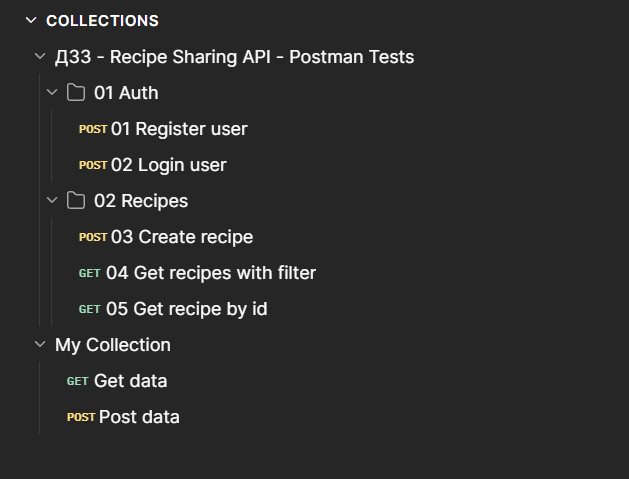
\includegraphics[width=0.7\textwidth]{images/collection.png}
    \caption{Структура коллекции Postman}
    \label{fig:collection}
\end{figure}

\subsection*{Настройка окружения Postman}

Для удобного запуска тестов было создано окружение \texttt{Recipe Sharing API Local Environment}. В окружении использовались переменные:

\begin{longtable}{|p{4cm}|p{9cm}|}
\hline
\textbf{Переменная} & \textbf{Назначение} \\
\hline
\texttt{baseUrl} & Базовый URL локального API: \texttt{http://localhost:8000/api} \\
\hline
\texttt{token} & JWT-токен, полученный после авторизации пользователя \\
\hline
\texttt{userId} & Идентификатор авторизованного пользователя \\
\hline
\texttt{recipeId} & Идентификатор рецепта, созданного во время выполнения сценария \\
\hline
\end{longtable}

Переменные \texttt{token}, \texttt{userId} и \texttt{recipeId} заполняются автоматически в ходе выполнения запросов. Это позволяет связывать запросы между собой и запускать коллекцию как единый сценарий.

\subsection*{Сценарий тестирования}

В итоговый сценарий вошли следующие запросы:

\begin{longtable}{|p{1cm}|p{4cm}|p{3cm}|p{5cm}|}
\hline
\textbf{№} & \textbf{Запрос} & \textbf{Метод и URL} & \textbf{Назначение} \\
\hline
1 & Register user & \texttt{POST /auth/register} & Регистрация тестового пользователя \\
\hline
2 & Login user & \texttt{POST /auth/login} & Авторизация пользователя и получение JWT-токена \\
\hline
3 & Create recipe & \texttt{POST /recipes} & Создание нового рецепта от имени пользователя \\
\hline
4 & Get recipes with filter & \texttt{GET /recipes?difficulty=easy} & Получение списка рецептов с фильтрацией по сложности \\
\hline
5 & Get recipe by id & \texttt{GET /recipes/\{recipeId\}} & Получение информации о рецепте по идентификатору \\
\hline
\end{longtable}

\subsection*{Регистрация пользователя}

Первым шагом выполняется регистрация пользователя. В теле запроса передаются имя, фамилия, имя пользователя, email и пароль.

Для запроса регистрации были добавлены проверки статуса ответа, формата JSON и наличия сообщения в ответе сервера.

\begin{lstlisting}[language=JavaScript, caption={Пример тестов для запроса регистрации}]
pm.test("Status code is 200", function () {
    pm.response.to.have.status(200);
});

const response = pm.response.json();

pm.test("Response is JSON object", function () {
    pm.expect(response).to.be.an("object");
});

pm.test("Response contains message", function () {
    pm.expect(response.message).to.exist;
});
\end{lstlisting}

\subsection*{Авторизация пользователя}

После регистрации выполняется вход пользователя в систему. В результате сервер возвращает \texttt{accessToken} и объект пользователя. Полученный токен сохраняется в переменную коллекции и используется в последующих запросах.

\begin{lstlisting}[language=JavaScript, caption={Сохранение токена и идентификатора пользователя}]
const response = pm.response.json();

pm.test("Access token exists", function () {
    pm.expect(response.accessToken).to.exist;
});

pm.test("User id exists", function () {
    pm.expect(response.user.id).to.exist;
});

pm.collectionVariables.set("token", response.accessToken);
pm.collectionVariables.set("userId", response.user.id);
\end{lstlisting}

На рисунке~\ref{fig:login} показан результат выполнения запроса авторизации. В ответе присутствуют JWT-токен и данные пользователя.

\begin{figure}[H]
    \centering
    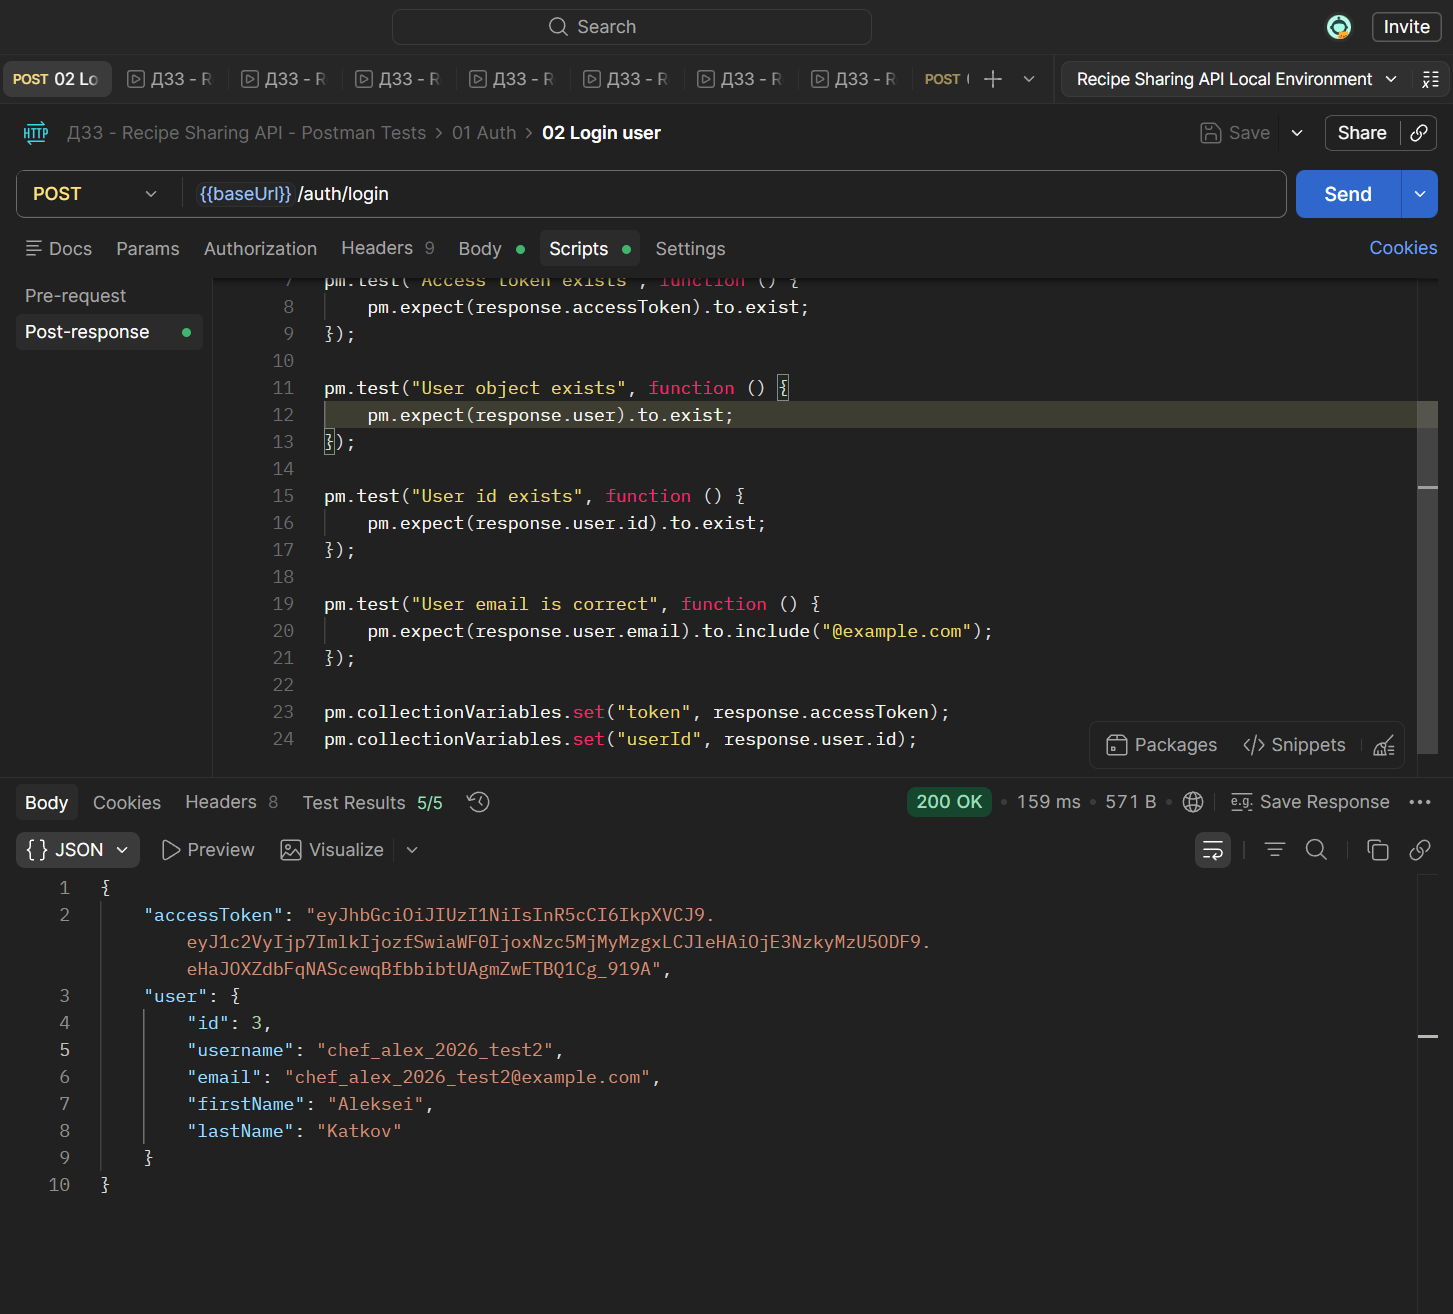
\includegraphics[width=0.95\textwidth]{images/login.png}
    \caption{Запрос авторизации пользователя и получение JWT-токена}
    \label{fig:login}
\end{figure}

\subsection*{Создание рецепта}

После авторизации выполняется создание рецепта. В тело запроса передаются название, описание, сложность, время приготовления, количество порций и идентификатор автора.

Для запроса создания рецепта проверяется:

\begin{itemize}
    \item успешный HTTP-статус;
    \item наличие идентификатора рецепта;
    \item корректность названия рецепта;
    \item корректность сложности рецепта;
    \item наличие автора рецепта.
\end{itemize}

Также идентификатор созданного рецепта сохраняется в переменную \texttt{recipeId}.

\begin{lstlisting}[language=JavaScript, caption={Тесты для запроса создания рецепта}]
const response = pm.response.json();

pm.test("Status code is 200 or 201", function () {
    pm.expect(pm.response.code).to.be.oneOf([200, 201]);
});

pm.test("Recipe has id", function () {
    pm.expect(response.id).to.exist;
});

pm.test("Recipe title is correct", function () {
    pm.expect(response.title).to.eql("Паста с томатным соусом");
});

pm.test("Recipe difficulty is easy", function () {
    pm.expect(response.difficulty).to.eql("easy");
});

pm.collectionVariables.set("recipeId", response.id);
\end{lstlisting}

Результат создания рецепта представлен на рисунке~\ref{fig:create_recipe}.

\begin{figure}[H]
    \centering
    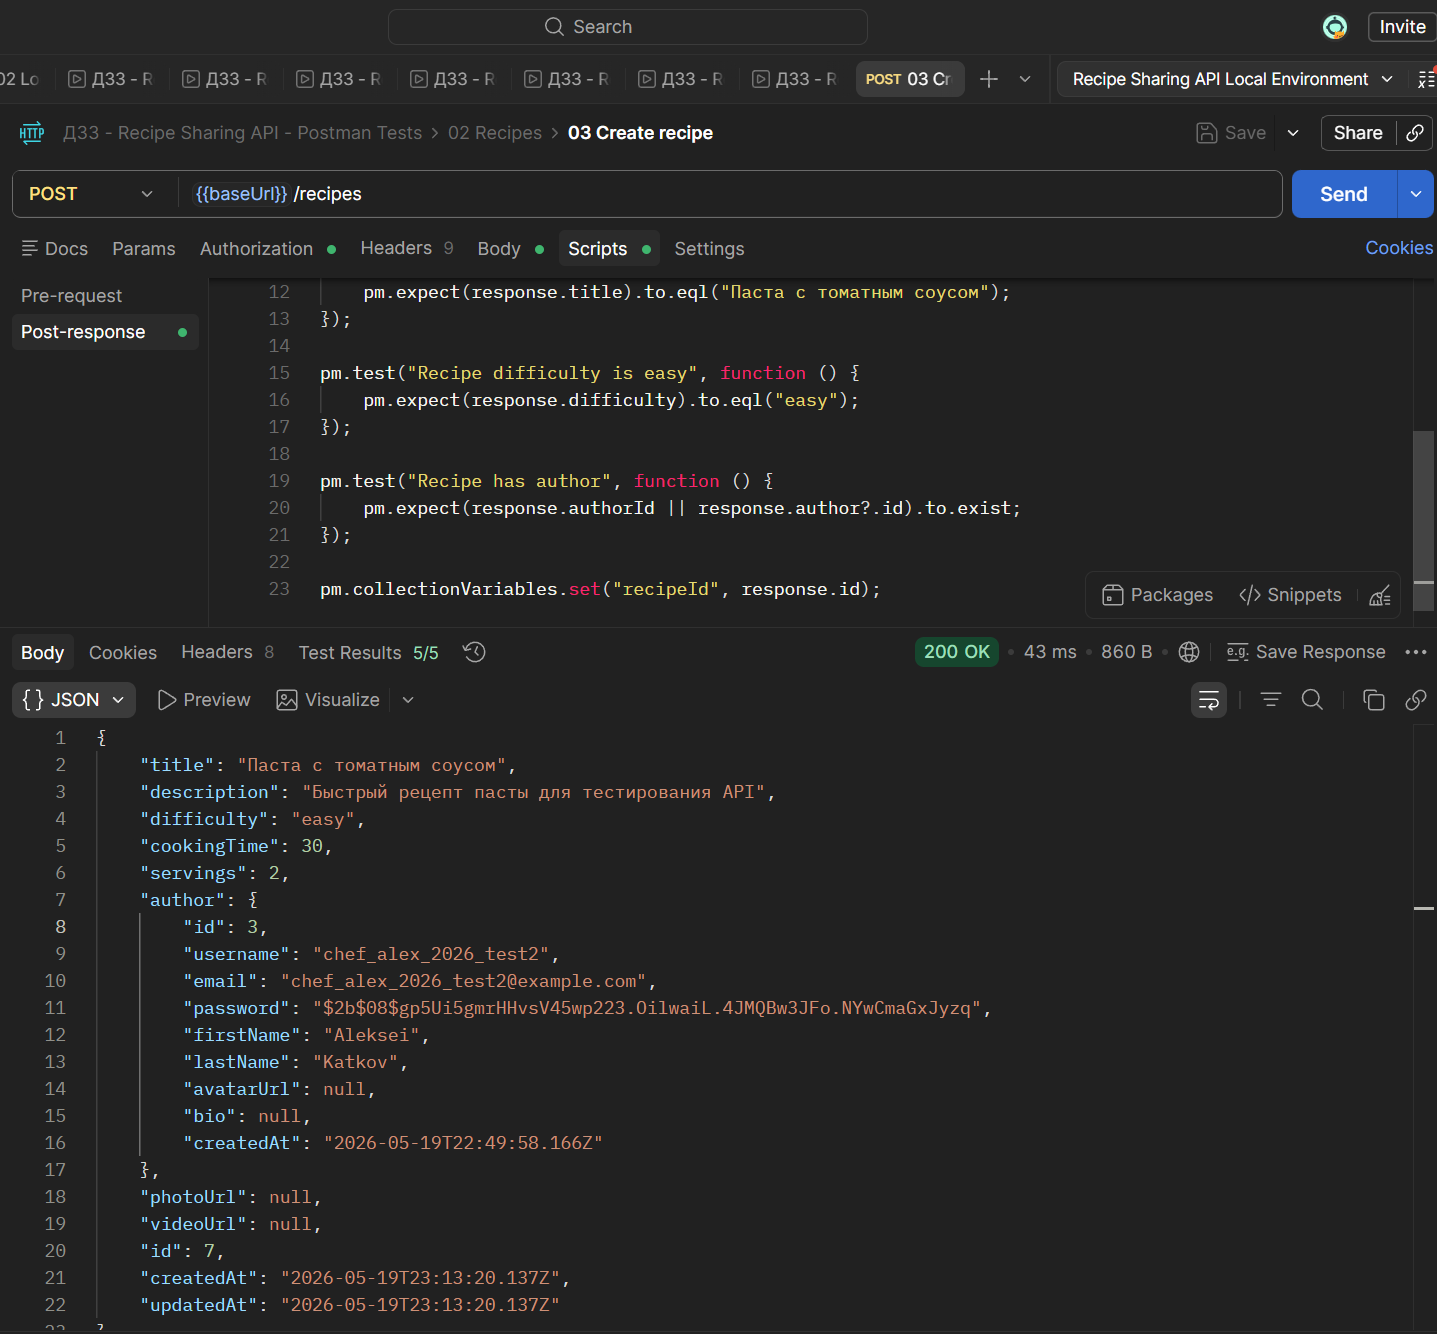
\includegraphics[width=0.95\textwidth]{images/create_recipe.png}
    \caption{Создание рецепта через Postman}
    \label{fig:create_recipe}
\end{figure}

\subsection*{Получение списка рецептов с фильтрацией}

Следующим шагом выполняется запрос списка рецептов с фильтрацией по сложности \texttt{easy}. Для запроса проверяется статус ответа, наличие ответа, корректность типа данных и наличие созданного рецепта в ответе.

\begin{lstlisting}[language=JavaScript, caption={Тесты для получения списка рецептов}]
pm.test("Status code is 200", function () {
    pm.response.to.have.status(200);
});

const response = pm.response.json();

pm.test("Response exists", function () {
    pm.expect(response).to.exist;
});

pm.test("Response is array or object", function () {
    pm.expect(response).to.satisfy(function (data) {
        return Array.isArray(data) || typeof data === "object";
    });
});

pm.test("Response contains created recipe data", function () {
    const text = JSON.stringify(response);
    pm.expect(text).to.include("Паста с томатным соусом");
});
\end{lstlisting}

Результат выполнения запроса показан на рисунке~\ref{fig:recipes_filter}.

\begin{figure}[H]
    \centering
    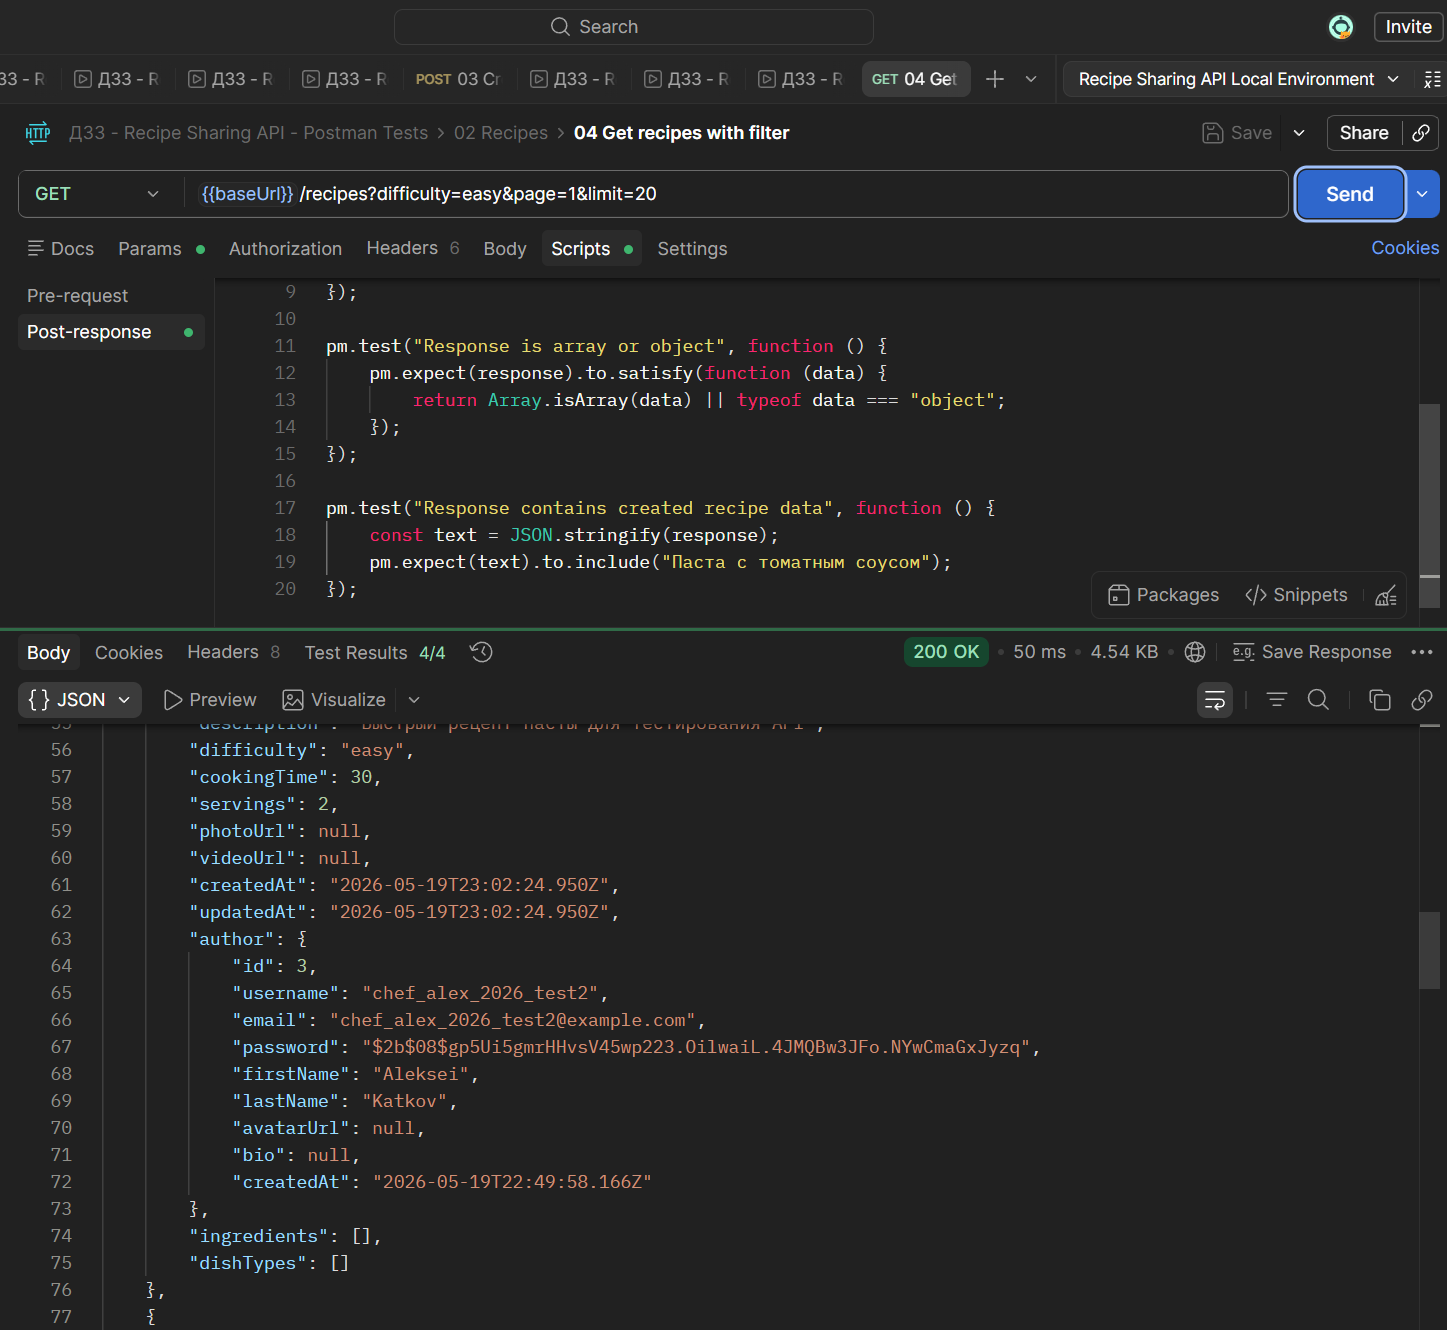
\includegraphics[width=0.95\textwidth]{images/recipes_filter.png}
    \caption{Получение списка рецептов с фильтрацией}
    \label{fig:recipes_filter}
\end{figure}

\subsection*{Получение рецепта по идентификатору}

Последним шагом сценария выполняется запрос получения данных о рецепте. Для запроса проверяется успешный HTTP-статус, наличие ответа и наличие данных созданного рецепта.

\begin{lstlisting}[language=JavaScript, caption={Тесты для получения рецепта по идентификатору}]
pm.test("Status code is 200", function () {
    pm.response.to.have.status(200);
});

const response = pm.response.json();

pm.test("Response exists", function () {
    pm.expect(response).to.exist;
});

pm.test("Response contains recipe data", function () {
    const text = JSON.stringify(response);
    pm.expect(text).to.include("Паста с томатным соусом");
});
\end{lstlisting}

Результат выполнения запроса представлен на рисунке~\ref{fig:recipe_by_id}.

\begin{figure}[H]
    \centering
    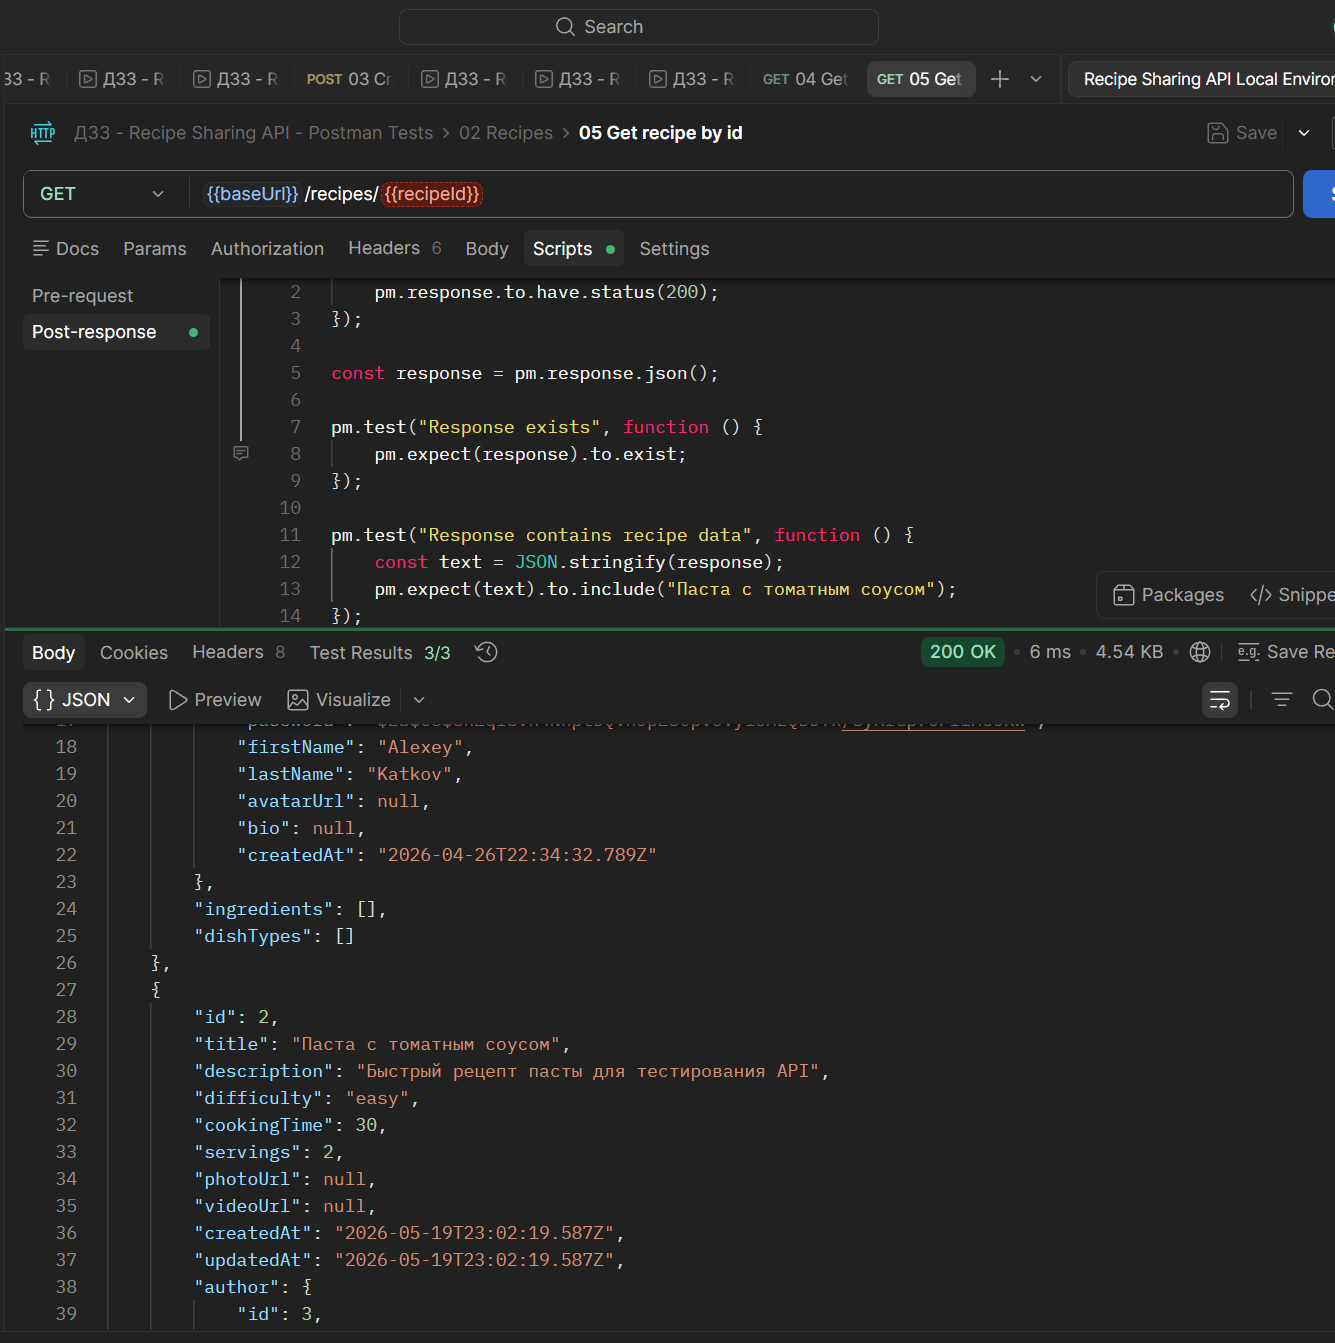
\includegraphics[width=0.95\textwidth]{images/recipe_by_id.png}
    \caption{Получение данных рецепта}
    \label{fig:recipe_by_id}
\end{figure}

\subsection*{Результаты запуска коллекции}

После настройки всех запросов коллекция была запущена через Collection Runner. Всего было выполнено 20 проверок. Все проверки завершились успешно: \texttt{20 passed}, \texttt{0 failed}, \texttt{0 errors}.

Результат запуска коллекции представлен на рисунке~\ref{fig:runner}.

\begin{figure}[H]
    \centering
    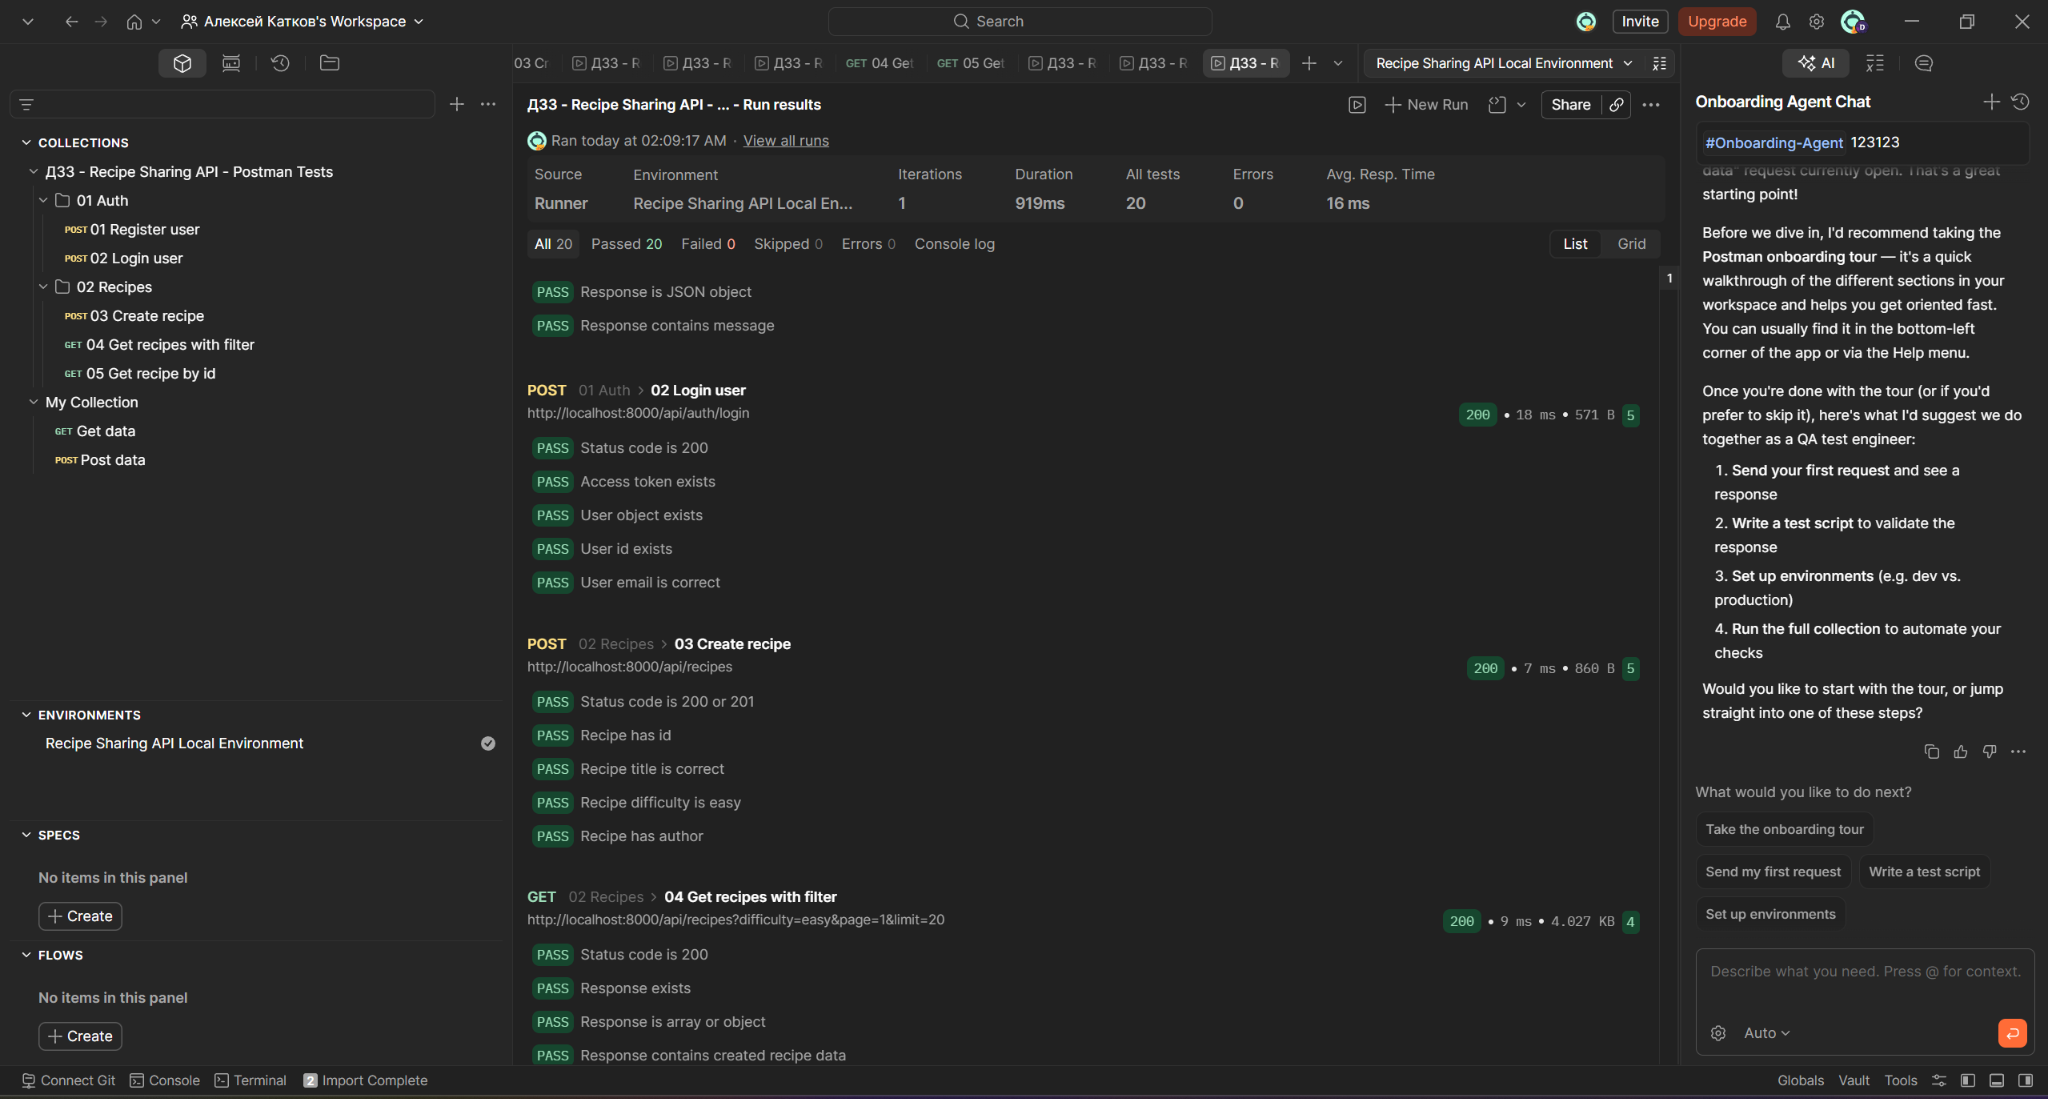
\includegraphics[width=0.95\textwidth]{images/runner.png}
    \caption{Успешный запуск коллекции Postman}
    \label{fig:runner}
\end{figure}

\section*{Вывод}

В ходе выполнения домашнего задания было реализовано тестирование API сервиса обмена рецептами средствами Postman. Был создан комплексный пользовательский сценарий, включающий регистрацию пользователя, авторизацию, создание рецепта, получение списка рецептов с фильтрацией и получение данных о рецепте.

В Postman были настроены переменные окружения и переменные коллекции, что позволило автоматически передавать данные между запросами: JWT-токен, идентификатор пользователя и идентификатор созданного рецепта.

Для каждого запроса были написаны автотесты, проверяющие HTTP-статусы, наличие нужных полей в ответе, корректность данных и связность сценария. Итоговый запуск коллекции показал успешное прохождение всех тестов: 20 проверок выполнены без ошибок.

Таким образом, основной процесс работы API был протестирован, а созданная коллекция Postman может использоваться для повторной проверки работоспособности серверной части приложения.

\end{document}
